%!TEX root = ../Hardtung_BA_SoSe20.tex

\section{Evaluating Origrammer}
\label{sec:evaluation}

To begin the evaluation process the 10 usability heuristics by Jakob Nielsen \cite{10usability_heuristics} will be used in order to facilitate a base, on which can be build upon with other evaluation methods if required. As established in \ref{sec:evaluationMethods}, the Usabilty Heuristics sometimes only identify problems without providing direct solutions. This is why this chapter will focus on finding problems and shortcomings of the Origrammer first. Afterwards, solutions can be developed that optimally fix most, or all, discovered issues without contradicting or counteracting other measures.

%Should i include Covid-19 problems in the bachelor thesis?
As the current (at the time of writing this thesis) Covid-19 pandemic hinders user involvement for the evaluation process, other measures have to be taken to ensure maximum efficiency and thoroughness. This is why there is an exhaustive list of all parts and features of the Origrammer below. Figure \ref{fig:origrammerMain} roughly shows what features are located where on the Origrammer.

\begin{figure}[htbp]
	\centering
	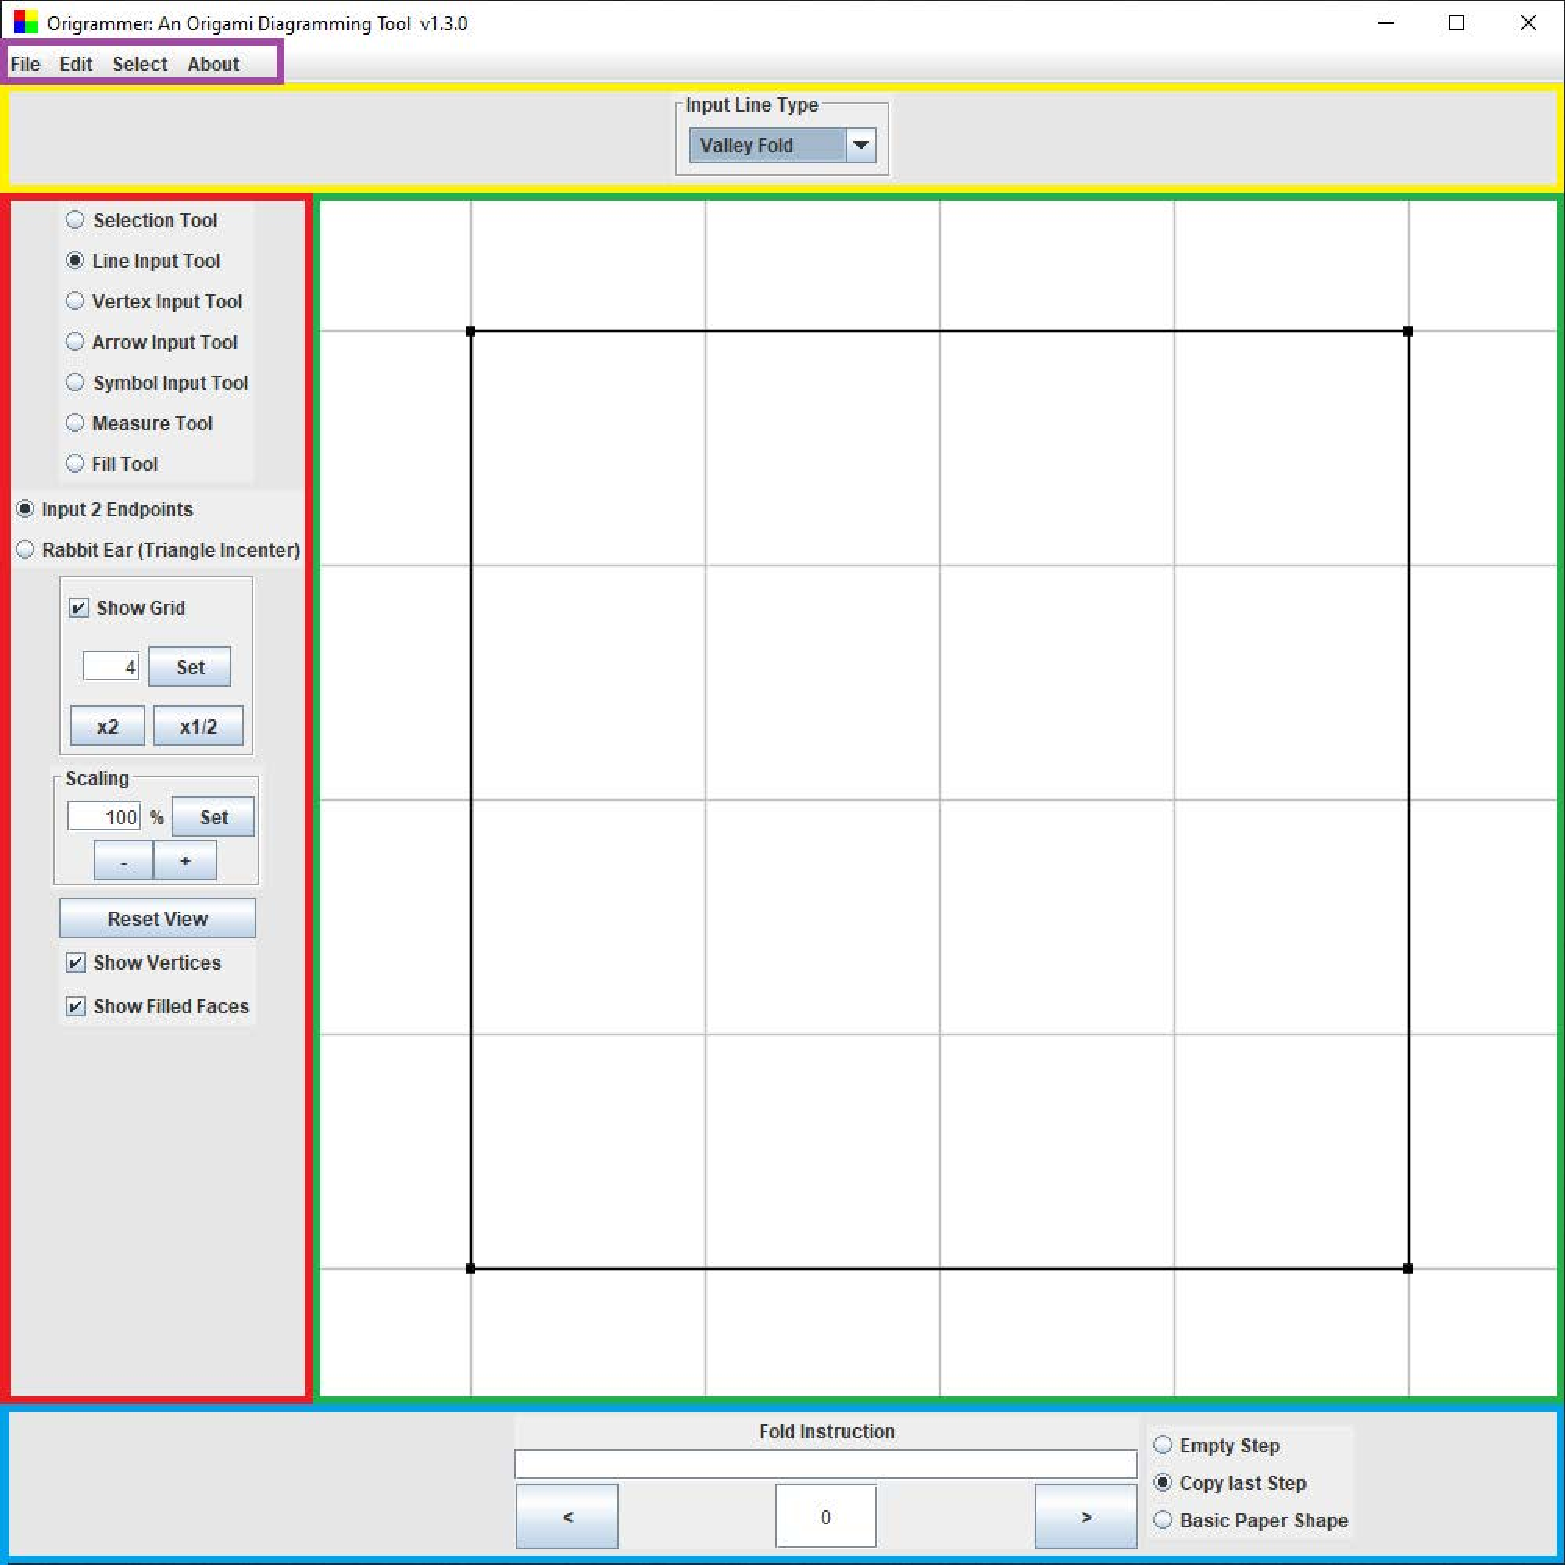
\includegraphics[width=0.8\textwidth]{OrigrammerMainParts}
	\caption{Menu Bar (Purple), Top Panel (Yellow), Side Panel (Red), Editing Panel (Green), Navigation Panel (Blue)}
	\label{fig:origrammerMain}
\end{figure}

\subsection{Origrammer Feature List}
\label{sec:featureList}

\begin{enumerate}
\item \textbf{Menu Bar (Purple)}

\begin{tabular}{l l l}
(a) New File & (b) Open File & (c) Save File \\
\emph{(d) Export File} & (e) Model Preferences & (f) Origrammer Preferences \\
\end{tabular}

\item \textbf{Side Bar (Red)}
    \begin{enumerate}
        \item Selection Tool \\
        \begin{tabular}{l l l}
        1. Click to Select & 2. Hover over Object & 3. Rectangular Selection \\
        \end{tabular}
        \item Line Input \\
        \begin{tabular}{l l}
        1. Two Point Input & 2. Triangle Incenter \\
        \end{tabular}
        \item Vertex Input \\
        \begin{tabular}{l l}
        1. Absolute Position & 2. Fraction of a Line \\
        \end{tabular}
        \item Arrow Input \\
        \begin{tabular}{l l l}
        1. Valley Fold & 2. Mountain Fold & 3. Turn over \\
        4. Push Here & 5. Pull out & 6. Inflate here \\
        \end{tabular}
        \item Symbol Input \\
        \begin{tabular}{l l l}
        1. Leader & 2. Repetition Box & 3. Next View Here \\
        4. Rotations & 5. Hold Here & 6. Hold Here and Pull \\
        7. X-Ray Circle & \emph{8. Fold Over \& Over} & 9. Equal Distances \\
        10. Equal Angles & 11. Crimps & 12. Pleats \\
        13. Closed Sinks
        \end{tabular}
        \item Measure Tool \\
        \begin{tabular}{l l l}
        1. Measure Length & 2. Measure Angle \\
        \end{tabular}
        \item Fill Tool
        \item Grid Settings
        \item Scaling Settings
    \end{enumerate}
\item \textbf{Navigation Panel (Blue)} \\
\begin{tabular}{l l l}
1. Fold Instructions & 2. Step Navigation & 3. New Step Options \\
\end{tabular}
\item \textbf{Top Panel (Yellow)} \\
See Side Panel for related features, as options for the selected Side Panel Tools appear on the Top Panel.
\item \textbf{Editing Panel (Green)} \\
See Side Panel for related features, as the selected Side Panel Tools are being used on the Editing Panel.
\end{enumerate}


\subsection{10 Usability Heuristics}
\label{sec:usabilityHeuristics}

With the Origrammer Feature List as a basis, the evalutation using the 10 Usability Heuristics can be carried out. Every feature from the list will be checked against all 10 heuristics in order to try and maximise the completeness of the result. The found usability issues will then lead to the planning of potential usability improvements.




\subsubsection*{1. Visibility of System Status}
\label{sec:visibility}

        \begin{tabular}{l | p{0.2\textwidth} | c | p{0.5\textwidth}}
        Nr: & Affects & Impact & Description \\ \hline
        1.01 & 2.b; 2.d-2.g & 3 & When an action requires multiple input points (e.g. placing a Fold Line by two endpoints), the user doesn't know where he is in the process. \\ \hline %maybe progressbar 
        1.02 & 2.d; 2.e & 7 & Always show a preview of the \texttt{OriArrow} or \texttt{OriSymbol} before final placing\\ \hline
        1.03 & 3.2; 3.3 & 6 & The user doesn't know how many diagram steps there are overall and where they are\\ \hline
        \end{tabular}



\subsubsection*{2. Aesthetic and Minimalist Design}
        \begin{tabular}{l | p{0.2\textwidth} | c | p{0.5\textwidth}}
        Nr: & Affects & Impact & Description \\ \hline
        2.01 & 2.a-2.i  & 4 &  The text in the Tool Selection on the Side Panel should be replaced by icons\\ \hline 
	2.02 & 4 & 3 & The text in the TopPanel for input and editing options should be replaced by icons\\ \hline
	2.03 & 2.f; 3 & 6 & The User Interface should always fit properly (is currently not fitting in the SidePanel for MeasureTool \& for some settings in the TopPanel)\\ \hline
        \end{tabular}

\subsubsection*{3. User Control and Freedom}

        \begin{tabular}{l | p{0.2\textwidth} | c | p{0.5\textwidth}}
        Nr: & Affects & Impact & Description \\ \hline
        3.01 & 2.a; 2.b; 2.d; 2.e; 2.g  & 5 & User should always be able to cancel an action (e.g. when inputting an object with multiple input points) )\\ \hline
        3.02 & 3.2; 3.3 & 8 & Navigating through the diagram steps is unflexible and slow\\ \hline 
        \end{tabular}


\subsubsection*{4. Consistency and Standards}

        \begin{tabular}{l | p{0.2\textwidth} | c | p{0.5\textwidth}}
        Nr: & Affects & Impact & Description \\ \hline
        4.01 & 2.a; 2.b; 2.d; 2.e; 2.g  & 2 & Editing options on the TopPanel should be labeled correctly (consistent naming scheme needed)\\ \hline 
	4.02 & 2.a; 4; 5 & 6 & When selecting and editing Symbols/Arrows make it consistent (e.g. when selecting different OriObject types like OriArrows and OriSymbols at the same time, the TopPanel overfills) \\ \hline
	4.03 & 1; 2; 3; 4 & 6 & UI elements should have consistent sizes (e.g. ``Set'' Buttons, \texttt{JTextFields})\\ \hline
	4.04 & 1; 2; 3; 4 & 4 & The sequential placement of UI parts should be consistent (e.g. for Input and Editing options on the TopPanel, have \texttt{JTextFields} first and then \texttt{JCheckBoxes} to the right\\ \hline
        \end{tabular}

\subsubsection*{5. Error Prevention}

        \begin{tabular}{l | p{0.2\textwidth} | c | p{0.5\textwidth}}
        Nr: & Affects & Impact & Description \\ \hline
        5.01 & 2.b.2 & 7 & Selecting the same point multiple times breaks the RabbitEar lines \\ \hline
        5.02 & 2.e.10  & 8 & Selecting points in the wrong order breaks inputs for the EqualAngle symbol \\ \hline 
        5.03 & 2.g & 7 & Selecting the same point multiple times breaks the FillTool \\ \hline
        5.04 & 1.a; 1.e; & 6 & Restrict the input of every JTextField (e.g. only allow numbers for number inputs)\\ \hline
        \end{tabular}
%Choose good default values for JTextField

\subsubsection*{6. Recognition Rather than Recall}

        \begin{tabular}{l | p{0.2\textwidth} | c | p{0.5\textwidth}}
        Nr: & Affects & Impact & Description \\ \hline
        6.01 & 2.f  & 5 & User should not be forced to remember the measured values (currently the measured values are being hidden, once the user selects a different tool from the SideBar)\\ \hline 
        \end{tabular}


\subsubsection*{7. Flexibility and Efficiency of Use}
        \begin{tabular}{l | p{0.2\textwidth} | c | p{0.5\textwidth}}
        Nr: & Affects & Impact & Description \\ \hline
        7.01 & 2.h & 3 & Give shortcuts for the Grid halve/ double buttons\\ \hline
        7.02 & 2.i  & 3 & Give shortcuts for the ResetView button\\ \hline
        7.03 & 2.i & 3 & Give shortcuts for the step by step zoom-in/zoom-out\\ \hline
        7.04 & 2.b & 8 & Give more Line Input options to avoid tedious work with grid adjustments\\ \hline
        7.05 & 2.d; 3; 4 & 8 & Give more flexibility when editing or placing arrows\\ \hline
        7.06 & 2.e; 3; 4 & 8 & Give more flexibility when editing or placing symbols\\ \hline
        7.07 & 3.2; 3.3 & 9 & The user can not change the order of steps, remove unwanted steps, or enter new steps between existing ones\\ \hline
        7.08 & 2.g & 7 & The user has to select the vertices by hand and is limited to triangles\\ \hline
        \end{tabular}

\subsubsection*{8. Recognition, Diagnosis and Recovery from Errors}
        \begin{tabular}{l | p{0.2\textwidth} | c | p{0.5\textwidth}}
        Nr: & Affects & Impact & Description \\ \hline
        8.01 & 2.b-2. & 5 & Error messages for wrong user inputs should be self-explanatory\\ \hline
        8.02 & 2.b-2.g & 4 & Error messages for wrong user inputs should explain how to fix the error\\ \hline
        \end{tabular}

\subsubsection*{9. Help and Documentation}
        \begin{tabular}{l | p{0.2\textwidth} | c | p{0.5\textwidth}}
        Nr: & Affects & Impact & Description \\ \hline
        9.01 & 2.a-2.i; 3; 4 & 6 & Show tooltips for all icons or non self-explanatory parts\\ \hline 
        9.02 & 2.a-2.g & 7 & Show short explanation on how inputs work for every possible input feature (could be combined with Nr.01 --> \ref{sec:visibility} Visibility\\ \hline
        \end{tabular}

\subsubsection*{10. Match between System and Real World}
        \begin{tabular}{l | p{0.2\textwidth} | c | p{0.5\textwidth}}
        Nr: & Affects & Impact & Description \\ \hline
        10.01 & 2.b-2.e & 5 & Use ``Origami terminology'' everywhere (e.g. Rabbit Ear instead of Triangle Incenter; Next View Here Symbol instead of Eye Symbol)\\ \hline
        \end{tabular}
